\section{Bayesian Linear Regression}
\begin{framed}
    \textbf{Closed form solutions}:
    $\vwhat_{\ls} = \inv{(\transpose{\mX} \mX)} \transpose{\mX} \vy$  \\
    $\vwhat_{\ridge} = \inv{(\transpose{\mX} \mX + \lambda \mI)} \transpose{\mX} \vy$
\end{framed}
\textbf{Notable Results}: $\Var{\vwhat_{\ls} \mid \rX} = \sigman^2(\transpose{\rX}\rX)^{-1}$ \\
A \textbf{Gaussian prior on the weights} $\vw \sim \N{\vzero}{\sigmap^2 \mI}$, yields the posterior distribution: $\log p(\vw \mid \vx_{1:n}, y_{1:n}) = -\frac{1}{2} \brackets*{\transpose{\vw}\mSigma^{-1}\vw - 2\vmu} + c$,
with $\mSigma \defeq \inv{\parentheses*{\sigman^{-2} \transpose{\mX} \mX + \sigmap^{-2} \mI}}$ and $\vmu \defeq \sigman^{-2} \mSigma \transpose{\mX} \vy$. 
We have $\vw \mid \vx_{1:n}, y_{1:n} \sim \N{\vmu}{\mSigma}$: \textit{Gaussians with known variance and linear likelihood} are self-conjugate. \\
MAP: $\vwhat_\MAP = \argmin_\vw \norm{\vy - \mX \vw}_2^2 + \frac{\sigman^2}{\sigmap^2} \norm{\vw}_2^2$, \textit{identical to ridge regression} with $\lambda \defeq \sigman^2 / \sigmap^2$. \\
\textbf{Laplace prior} $\leftrightarrow$ \textbf{lasso regr.} with ${\lambda \defeq \sigman^2 / \ell}$. \\
\textbf{Bayesian inference} \\
Distribution for a test point $\vxs$ is: $\ys \mid \vxs, \vx_{1:n}, y_{1:n} \sim \N{\transpose{\vmu} \vxs}{\transpose{\vxs} \mSigma \vxs + \sigman^2}$. \\
$\Var{\ys \mid \vxs} = \underbrace{\E[\vtheta]{\Var[\ys]{\ys \mid \vxs, \vtheta}}}_{\text{aleatoric uncertainty}} + \underbrace{\Var[\vtheta]{\E[\ys]{\ys \mid \vxs, \vtheta}}}_{\text{epistemic uncertainty}}$.\\
Aleatoric = noise in data; Epistemic = ``noise" in model. \\
For non-linear function $\vphi$: Define $\mPhi = \vphi(\rX)$, so-called \textbf{Kernel}. With a gaussian prior we get: $\vf \mid \mX \sim \N{\mPhi \E{\vw}}{\mPhi \Var{\vw} \transpose{\mPhi}} = \N{\vzero}{\mK}$, with $\mK = \sigmap^2 \mPhi \transpose{\mPhi}$. We define the \textbf{Kernel-function}: $k(\vx, \vxp) \defeq \sigmap^2 \cdot \transpose{\vphi(\vx)} \vphi(\vxp) = \Cov{f(\vx), f(\vxp)}$.
\begin{framed}
    \textbf{Linear Kernel}: $k(\vx, \vxp) = l \transpose{\vx} \vxp$ \\
    \textbf{RBF/Gaussian}: $k(\vx, \vxp) = \exp{-\frac{(\vx - \vxp)^2}{2 l^2}}$ \\
    \textbf{Polynomial Kernel} $k(\vx, \vxp) = (1 + \transpose{\vx} \vxp)^d$ \\
    \textbf{Laplacian Kernel}: $k(\vx, \vxp) = \exp{\left(- \norm{\vx - \vxp}/l\right)}$ \\
    (not diff'able/smooth)
\end{framed}
\begin{framed}
    \textbf{Properties of Kernels}:  \\
    Symmetry: $k(\vx, \vxp) = k(\vxp, \vx)$ and $\mK_{\sA\sA}$ is p.s.d. \\
    Kernels can be \textbf{composed} in the following ways to obtain a new kernel: addition, multiplication, positive scalar multiplication and composition with a funtion $f$ if $f$ is polynomial with positive coefficients or $\exp$.
\end{framed}
\textbf{Stationary} if $\exists\tilde{k}$ s.t. $\tilde{k}(\vx - \vxp) = k(\vx, \vxp)$ \\
and \textbf{Isotropic} if $\exists\tilde{k}$ s.t. $\tilde{k}(\norm{\vx-\vxp}_2) = k(\vx, \vxp)$. \\ 
\textbf{Kalman Filters} \\
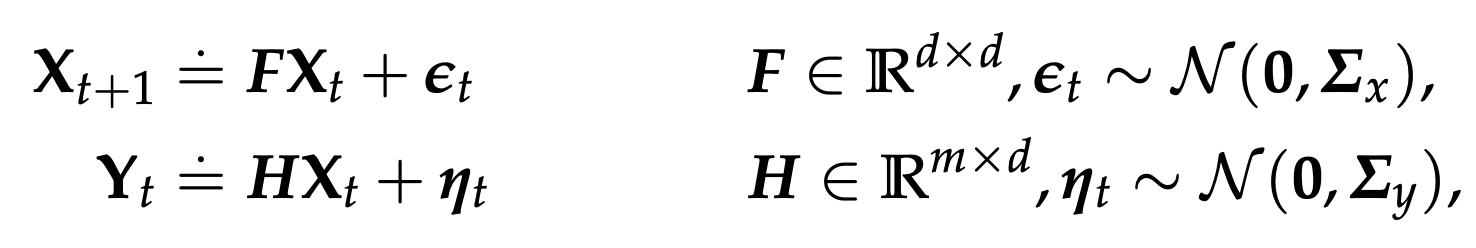
\includegraphics[width=0.8\linewidth]{images/kalman 1.png}
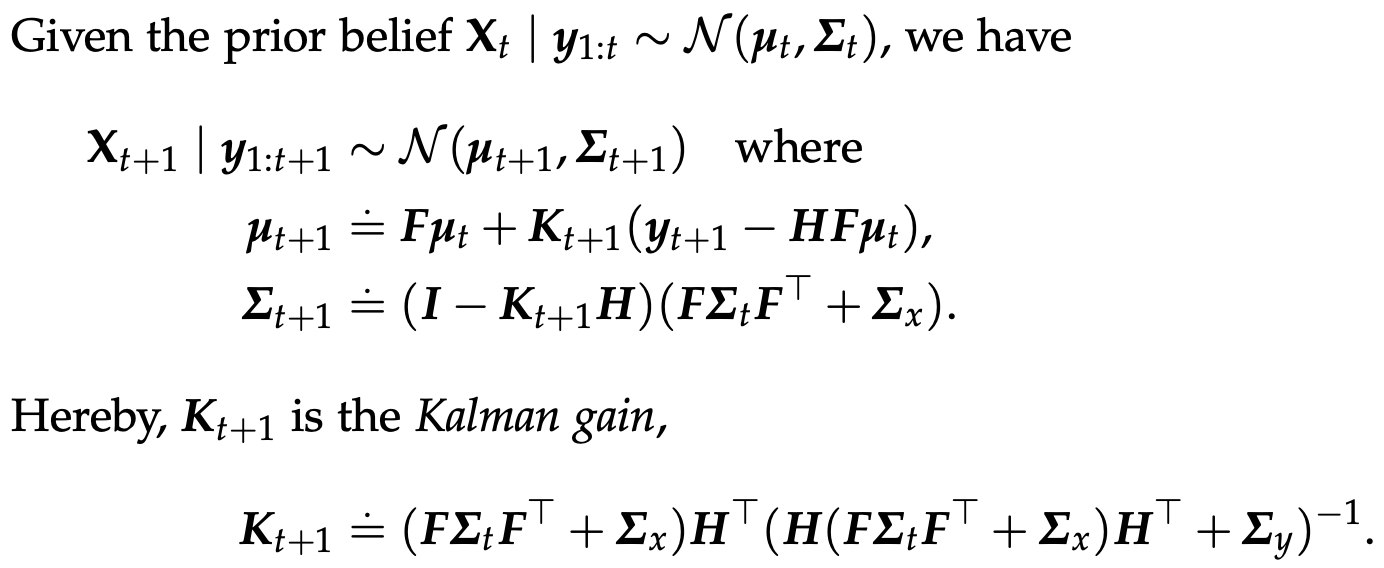
\includegraphics[width=\linewidth]{images/kalman 2.png}
